\chapter{Modello di qualit\`{a}} \label{chap:modello_qualità}

	Abbiamo visto nel primo capitolo come valutare l'usabilità di un sito tramite il metodo di valutazione euristica. Tuttavia  l'usabilità, per quanto importante, non rappresenta l'unico aspetto di un sito web. Per questo Roberto Polillo ha proposto un metodo secondo il quale valutare la ``qualità'' di un sito web e poterlo poi confrontare con altri siti simili.\\
	\\
	Questo modello prevede di assegnare ad ogni sito un voto, in una scala da 0 a 4, secondo 7 caratteristiche da lui  individuate, che sono le seguenti:
	\begin{itemize}
		\item Architettura
		\item Comunicazione
		\item Funzionalità
		\item Contenuto
		\item Gestione
		\item Accessibilità
		\item Usabilità
		\item Modello di qualità
	\end{itemize}
	Ma questa è soltanto la prima e più generica formulazione del suo modello. Se si volesse infatti andare più nel dettaglio e costruire un modello più fedele, si può infatti scomporre ogni caratteristica in opportune sottocaratteristiche e quindi valutare il sito (o i siti) in base ad esse.\\
	\\
	Una volta assegnati i voti alle varie caratteristiche o sottocaratteristiche si potranno facilmente confrontare due o più siti semplicemente confrontando i valori ottenuti. Uno strumento utile in questo senso sono i diagrammi a stella, che permettono, a colpo d'occhio, di vedere quale sito sia migliore degli altri secondo le diverse caratteristiche.\\
	\\
	Andiamo a vedere adesso quanto sono ``buoni'' Gmail e Yahoo Mail secondo le caratteristiche previste dal modello.

	\section{Architettura} \label{sec:architettura}
	
		L'architettura, come sostiene opportunamente Polillo \cite{polillo:modello}, può essere definita come ``la struttura generale del sito e le modalità di navigazione che esso rende disponibili ai propri utenti''. In particolare, la struttura del sito verrà analizzata ``in funzione dei suoi contenuti informativi'' e non in base alla sua ``architettura interna''. È possibile, infatti, individuare le tre seguenti sottocaratteristiche con cui valutare al meglio l'architettura di un sito web, ossia: la \textit{struttura}, la \textit{mappa del sito} e la \textit{navigazione}.\\
		\\
		La \textbf{struttura} del sito è adeguatamente ben definita sia in Gmail che in Yahoo Mail. Le varie cartelle della posta elettronica, infatti, si trovano sempre sulla parte sinistra dello schermo, la lista delle mail appare al centro della pagina ed è dunque ben visibile all'utente e, infine, le operazioni di composizione inerenti alle varie mail si trovano sempre nello spazio soprastante le mail stesse. Indipendentemente dalla pagina della posta elettronica che l'utente visiterà, la struttura del sito rimarrà invariata e ben definita in entrambi i provider di posta. Assegnamo, per questo motivo, $4/4$ ad entrambi i siti.\\
		\\
		Naturalmente, parlando di provider della posta elettronica, non è necessaria alcuna \textbf{mappa del sito} per orientare più facilmente l'utente poiché, come sottolineato precedentemente, la struttura informativa dei due siti permette all'utente di orientarsi facilmente all'interno del sito web. Nel caso l'utente necessiti di un aiuto aggiuntivo, allora sia Gmail che Yahoo Mail forniscono una ``guida'' o ``help'' all'utente tramite il menù delle impostazioni. Attribuiamo allora un voto di $0/4$ ad entrambi, ma anche un peso $0$ alla mappa del sito.\\
		\\
		La \textbf{navigazione}, invece, è implementata in maniera differente nei due provider di posta. In particolar modo, analizzando concetti chiave come il supporto o meno di tasti rapidi, la possibilità di navigare con tastiera e la presenza del tasto ``Indietro'', è possibile notare come risulti più adeguata la navigazione in Gmail rispetto alla navigazione in Yahoo Mail (come visto in Sezione \ref{sec:controllo_libertà}). Diamo allora $4/4$ a Gmail e $2/4$ a Yahoo Mail.
	
	\section{Comunicazione} \label{sec:comunicazione}
	
		Si parla di comunicazione, invece, quando ci si riferisce ``alla chiarezza con cui il sito comunica il suo scopo, alla sua coerenza con l'immagine dell'organizzazione titolare del sito, all'attrattiva grafica ed, infine, alla relazione che instaura con gli utenti'' \cite{polillo:modello}. È possibile, dunque, individuare le tre seguenti sottocaratteristiche: \textit{home page}, \textit{brand image} e \textit{grafica}.\\
		\\
		Sia la \textbf{home page} che la \textbf{brand image} sono adeguatamente ben definiti e rispettati in entrambi i provider di posta elettronica (Gmail e Yahoo Mail). Mentre la home page comunica chiaramente gli obiettivi del sito, infatti, è possibile notare come anche lo stile ed i colori dei due siti siano coerenti col provider di posta a cui si fa riferimento. Per questo assegnamo $4/4$ ad entrambi i siti nelle due sottocaratteristiche.\\
		\\
		La \textbf{grafica} di Gmail, invece, è migliore rispetto alla grafica di Yahoo Mail. Come sottolineato anche all'interno della Sezione \ref{sec:design_estetica_minimalista}, infatti, Gmail contiene alcuni accorgimenti che lo fanno preferire a Yahoo Mail dal punto di vista grafico come, ad esempio, la minimizzazione iniziale del menù laterale facente riferimento alle varie cartelle della posta elettronica. Per questo attribuiamo $4/4$ a Gmail e $3.5/4$ a Yahoo Mail.
	
	\section{Funzionalit\`{a}} \label{sec:funzionalità}
	
		Con il concetto di funzionalità, invece, si intende ``l'insieme delle funzioni che il sito mette a disposizione dei propri utenti. Da questo punto di vista, un sito è di qualità quando supporta bene l'utente nello svolgimento delle funzioni che gli servono, e tutte queste sono realizzate in modo corretto dal software, cioè senza errori.'' \cite{polillo:modello} In particolare, verranno valutate l'\textit{adeguatezza} e la \textit{correttezza} di tali funzioni.\\
		\\
		Per quanto riguarda l'\textbf{adeguatezza}, in Yahoo Mail, a differenza di Gmail, non viene supportata la funzione di etichettatura e, dunque, il sistema non permette all'utente di etichettare le varie mail presenti nella propria casella di posta elettronica. A causa di questa mancanza assegnamo $4/4$ a Gmail e $3/4$ a Yahoo Mail.\\
		\\
		Invece, per ciò che concerne la \textbf{correttezza} delle funzioni implementate in Gmail e in Yahoo Mail, non è possibile notare alcuna inefficienza. Assegnamo perciò $4/4$ ad entrambi.
	
	\section{Contenuto} \label{sec:contenuto}
	
		La quarta caratteristica introdotta da Polillo fa riferimento alla ``qualità dei vari contenuti informativi di un sito web, considerando aspetti come l'affidabilità, il livello di aggiornamento, la comprensibilità del linguaggio, \dots'' \cite{polillo:modello}. È possibile, dunque, distinguere quattro differenti sottocaratteristiche: la \textit{categorizzazione} (o \textit{labeling}), lo \textit{stile}, l'\textit{informazione} e la \textit{localizzazione}.\\
		\\
		La \textbf{categorizzazione} (o \textbf{labeling}), come già ampiamente sostenuto nella valutazione euristica dei due siti web, è presente in Gmail mentre non è stata attualmente implementata in Yahoo Mail, che fornisce soltanto un sistema di cartelle. Per questo attribuiamo $4/4$ a Gmail e $2/4$ a Yahoo Mail.\\
		\\
		Lo \textbf{stile} del testo delle varie email è adeguato in entrambi i provider di posta elettronica. Tuttavia, Gmail consente di modificare opportunamente lo stile di testo specificando anche il colore desiderato, oltre al font ed alla dimensione del testo. Yahoo Mail, invece, consente di modificare lo stile di testo dei vari messaggi di posta, ma non consente di specificare il colore del testo desiderato. Assegnamo allora $4/4$ a Gmail e $3.5/4$ a Yahoo Mail.\\
		\\
		I concetti di \textbf{informazione} e \textbf{localizzazione}, invece, sono adeguatamente ben implementati e corretti in entrambi i provider di posta elettronica. I voti per queste due sottocaratteristiche sono di $4/4$ per entrambi i siti.
	
	\section{Gestione} \label{sec:gestione}
	
		Con gestione di un sito si intende come esso viene gestito dai suoi amministratori in modo da fornire all'utente un servizio sempre migliore.\\
		\\
		Per quanto riguarda la \textbf{disponibilità} del sito stesso (quanto poco il sito risulta down, ad esempio) entrambi i siti sono molto ben equipaggiati per far fronte a questo tipo di situazione e non ci è mai capitato di non poter accedere  all'uno o all'altro: assegnamo $4/4$ ad entrambi.\\
		\\
		Con \textbf{monitoraggio} invece si intende che le azioni svolte dall'utente siano opportunamente monitorate dal sistema in modo da evitare danni o errori. In questo caso, come già visto, è molto difficile  produrre errori e tutte le azioni eseguite dall'utente sono seguite in entrambi i siti: assegnamo $4/4$ ad entrambi.\\
		\\
		L'\textbf{aggiornamento} di entrambi i provider è risultato piuttosto continuo ed efficace negli ultimi anni. Certe volte si è trattato di semplici aggiornamenti grafici o stilistici,  mentre altre volte è stato rivoluzionato completamente il sito. In ogni caso, gli aggiornamenti hanno sempre portato a dei miglioramenti del sito stesso. Anche in questo caso assegnamo $4/4$ ad entrambi.\\
		\\
		Riguardo la \textbf{relazione con gli utenti} ricordiamo la guida di Gmail e di Yahoo Mail e possiamo aggiungere che da entrambe le guide è possibile accedere a forum/aiuti in linea dove altre persone (personale di supporto o anche altri utenti) possono aiutarci a risolvere un dubbio o un problema col sito, qualora non fosse reperibile nella guida. Attribuiamo $4/4$ a Gmail e $3/4$ a Yahoo Mail, per il semplice fatto che in Yahoo Mail la  guida e i vari contatti sono posti in un sito separato e non integrati con la casella di posta stessa (come visto in Sezione \ref{sec:documentazione}).
	
	\section{Accessibilit\`{a}} \label{sec:accessibilità}
	
		L'accessibilità si occupa di tutti quegli aspetti che permettono a tutti di accedere al sito velocemente e senza problemi.\\
		\\
		Il primo aspetto dell'accessibilità sono quindi i \textbf{tempi d'accesso}. Abbiamo già visto,  in Sezione \ref{sec:visibilità_stato_sistema}, come Gmail informi di più  l'utente durante le attese del sito, ovvero fornendo più informazione rispetto a Yahoo Mail sui tempi d'accesso. Avevamo anche fatto notare come Yahoo Mail sia meno reattivo rispetto a Gmail nel segnalare alcuni cambi di stato del sistema, come il salvataggio di una bozza. Per queste ragioni assegnamo $4/4$ a Gmail e $3/4$ a Yahoo Mail.\\
		\\
		Con \textbf{reperibilità} si intende invece quanto risulta facile all'utente trovare il sito. In entrambi i casi i siti risultano molto in vista ed è molto facile trovarli, sia tramite un qualsiasi motore di ricerca che da altri siti appartenenti alle stesse compagnie (ad esempio per raggiungere Gmail da un qualsiasi altro sito Google avremmo sempre un collegamento disponibile, solitamente in alto a destra della pagina). Per questo motivo assegnamo $4/4$ ad entrambi.\\
		\\
		Un altro aspetto in questo senso è l'\textbf{indipendenza dal browser}. Sia Gmail\footnote{\url{https://support.google.com/mail/answer/6557?hl=en}} che Yahoo Mail\footnote{\url{https://help.yahoo.com/kb/supported-browser-sln2929.html}} supportano ufficialmente le ultime versioni di Google Chrome, Firefox, Internet Explorer e Safari. Per browser e/o versioni non supportate, alcune funzionalità dei due siti potrebbero non essere disponibili. È vero che con quei 4 browser vengono coperti la maggior parte degli utenti, ma potrebbero esser stati  inclusi anche altri browser in ascesa, come Opera. Per questo motivo abbiamo assegnato un voto di $3/4$ ad entrambi. Tuttavia quest'aspetto non è di primaria importanza (è anche compito di un buon browser adeguarsi agli standard e visualizzare il numero maggiore di pagine possibile), per questo gli abbiamo attribuito un peso di $0.75$.\\
		\\
		Infine c'è l'aspetto dell'\textbf{accessibilità per i disabili}. In nessuno dei due siti abbiamo trovato funzionalità  per i disabili messe in bella vista o facilmente accessibili, anche se siamo convinti che entrambi forniscano in qualche modo degli aiuti per gli utenti disabili (ad esempio diverse modalità di visualizzazione per gli utenti ipovedenti). Per questo abbiamo attribuito un voto di $2/4$ ad entrambi ed un peso di $0.25$ a questa sottocaratteristica.
	
	\section{Usabilit\`{a}} \label{sec:usabilità}
	
		L'ultima caratteristica da prendere in considerazione è l'usabilità. Con usabilità si intende ``tutto ciò che rende il sito facile e gradevole da usare'' \cite{polillo:modello} ed essa non è il risultato di un'attività specifica,  ma di tutte le altre caratteristiche appena elencate.\\
		\\
		Avendo eseguito al capitolo precedente la valutazione euristica dell'usabilità, il valore di usabilità da attribuire ai due siti lo otteniamo direttamente sfruttando quello studio. Ci è bastato infatti trasformare i voti assegnati all'usabilità dei due siti (Capitolo \ref{chap:valutazione_euristica}, Sezione \ref{sec:valutazione_finale}, pagina \pageref{sec:valutazione_finale}) da voti in decimi a voti in quarti, ottenendo $3.92/4$ per Gmail e $3.16/4$ per Yahoo Mail.\\
		\\
		Polillo ha proposto, nel suo modello, di scomporre l'usabilità in 3 sottocaratteristiche, in particolare \textit{efficacia}, \textit{efficienza} e \textit{soddisfazione}. Tuttavia, per la natura estremamente soggettiva di queste sottocaratteristiche e per il fatto che avevamo già calcolato l'usabilità con il metodo di valutazione euristica,  abbiamo deciso qui di non suddividere l'usabilità in ulteriori sottocaratteristiche.
	
	\section{Modello di qualit\`{a}} \label{sec:modello_qualità}
	
		Prendiamo adesso tutti i voti e i pesi assegnati alle varie sottocaratteristiche dei due siti e costruiamo delle tabelle riassuntive. Una volta fatto questo, calcoliamo la  media pesata delle sottocaratteristiche di ogni caratteristica: in questo modo otterremo il voto pesato delle 7 caratteristiche dei due siti. Il risultato sono le Tabelle \ref{tab:valutazione_gmail} e \ref{tab:valutazione_yahoo}.
		\begin{table}[h!]
			\centering
			\begin{tabular}{|l|r|r|r|}
				\hline
				\multicolumn{1}{|c|}{Caratteristica} & \multicolumn{1}{c|}{Voto} & \multicolumn{1}{c|}{Peso} & \multicolumn{1}{c|}{Voto pesato}\\ \hline\hline
				\textbf{Architettura} & \textbf{4.00} & \textbf{2.00} & \textbf{4.00}\\ \hline
				Struttura & 4 & 1 & 4\\ \hline
				Mappa del  sito & 0 & 0 & 0\\ \hline
				Navigazione & 4 & 1 & 4\\ \hline
				\textbf{Comunicazione} & \textbf{4.00} & \textbf{3.00} & \textbf{4.00}\\ \hline
				Home page & 4 & 1 & 4\\ \hline
				Brand image & 4 & 1 & 4\\ \hline
				Grafica & 4 & 1 & 4\\ \hline
				\textbf{Funzionalità} & \textbf{4.00} & \textbf{2.00} & \textbf{4.00}\\ \hline
				Adeguatezza & 4 & 1 & 4\\ \hline
				Correttezza & 4 & 1 & 4\\ \hline
				\textbf{Contenuto} & \textbf{4.00} & \textbf{4.00} & \textbf{4.00}\\ \hline
				Categorizzazione/labeling & 4 & 1 & 4\\ \hline
				Stile & 4 & 1 & 4\\ \hline
				Informazione & 4 & 1 & 4\\ \hline
				Localizzazione & 4 & 1 & 4\\ \hline
				\textbf{Gestione} & \textbf{4.00} & \textbf{4.00} & \textbf{4.00}\\ \hline
				Disponibilità & 4 & 1 & 4\\ \hline
				Monitoraggio & 4 & 1 & 4\\ \hline
				Aggiornamento & 4 & 1 & 4\\ \hline
				Relazione con gli utenti & 4 & 1 & 4\\ \hline
				\textbf{Accessibilità} & \textbf{3.25} & \textbf{3.00} & \textbf{3.58}\\ \hline
				Tempi d'accesso & 4 & 1 & 4\\ \hline
				Reperibilità & 4 & 1 & 4\\ \hline
				Indipendenza dal browser & 3 & 0.75 & 2.25\\ \hline
				Accessibilità per i disabili & 2 & 0.25 & 0.5\\ \hline
				\textbf{Usabilità} & \textbf{3.92} & \textbf{1.00} & \textbf{3.92}\\ \hline
				Usabilità & 3.92 & 1 & 3.92\\ \hline
			\end{tabular}
			\caption[Valutazione di Gmail]{La valutazione di Gmail secondo le sue caratteristiche (in grassetto) e sottocaratteristiche.}
			\label{tab:valutazione_gmail}
		\end{table}
		\begin{table}[h!]
			\centering
			\begin{tabular}{|l|r|r|r|}
				\hline
				\multicolumn{1}{|c|}{Caratteristica} & \multicolumn{1}{c|}{Voto} & \multicolumn{1}{c|}{Peso} & \multicolumn{1}{c|}{Voto pesato}\\ \hline\hline
				\textbf{Architettura} & \textbf{2.00} & \textbf{2.00} & \textbf{3.00}\\ \hline
				Struttura & 4 & 1 & 4\\ \hline
				Mappa del  sito & 0 & 0 & 0\\ \hline
				Navigazione & 2 & 1 & 2\\ \hline
				\textbf{Comunicazione} & \textbf{3.83} & \textbf{3.00} & \textbf{3.83}\\ \hline
				Home page & 4 & 1 & 4\\ \hline
				Brand image & 4 & 1 & 4\\ \hline
				Grafica & 3.5 & 1 & 3.5\\ \hline
				\textbf{Funzionalità} & \textbf{3.50} & \textbf{2.00} & \textbf{3.50}\\ \hline
				Adeguatezza & 3 & 1 & 3\\ \hline
				Correttezza & 4 & 1 & 4\\ \hline
				\textbf{Contenuto} & \textbf{3.37} & \textbf{4.00} & \textbf{3.37}\\ \hline
				Categorizzazione/labeling & 2 & 1 & 2\\ \hline
				Stile & 3.5 & 1 & 3.5\\ \hline
				Informazione & 4 & 1 & 4\\ \hline
				Localizzazione & 4 & 1 & 4\\ \hline
				\textbf{Gestione} & \textbf{3.75} & \textbf{4.00} & \textbf{3.75}\\ \hline
				Disponibilità & 4 & 1 & 4\\ \hline
				Monitoraggio & 4 & 1 & 4\\ \hline
				Aggiornamento & 4 & 1 & 4\\ \hline
				Relazione con gli utenti & 3 & 1 & 3\\ \hline
				\textbf{Accessibilità} & \textbf{3.00} & \textbf{3.00} & \textbf{3.25}\\ \hline
				Tempi  d'accesso & 3 & 1 & 3\\ \hline
				Reperibilità & 4 & 1 & 4\\ \hline
				Indipendenza dal browser & 3 & 0.75 & 2.25\\ \hline
				Accessibilità per i disabili & 2 & 0.25 & 0.5\\ \hline
				\textbf{Usabilità} & \textbf{3.16} & \textbf{1.00} & \textbf{3.16}\\ \hline
				Usabilità & 3.16 & 1 & 3.16\\ \hline
			\end{tabular}
			\caption[Valutazione di Yahoo Mail]{La valutazione di Yahoo Mail secondo le sue caratteristiche (in grassetto) e sottocaratteristiche.}
			\label{tab:valutazione_yahoo}
		\end{table}
		\\
		
		Infine, raggruppando i voti delle caratteristiche o delle sottocaratteristiche dei due siti otteniamo, rispettivamente, i grafici in Figura \ref{fig:radar_chart} e in Figura \ref{fig:radar_chart_sottocaratteristiche}. Questi grafici sono detti ``diagrammi a stella'', ``grafici radar'' o ``grafi di Kiviat'' e rappresentano un modo per vedere a colpo d'occhio la bontà di un sito rispetto ad un altro secondo vari aspetti.\\
		Nel nostro caso vediamo subito come Yahoo Mail sia sempre contenuto in Gmail, pur rimanendo un valido provider di posta elettronica con voti mediamente alti.
		\begin{figure}[h!]
			\begin{center}
				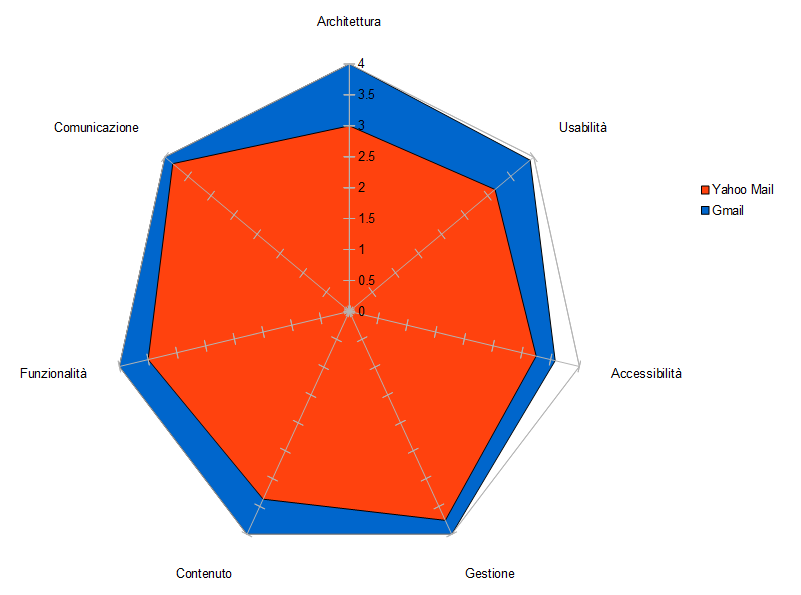
\includegraphics[scale=0.6]{radar_chart_filled.png}
			\end{center}
			\caption[Diagramma a stella]{Diagramma a stella che confronta Gmail e Yahoo Mail secondo le 7 caratteristiche principali individuate da Polillo, con i voti pesati delle Tabelle \ref{tab:valutazione_gmail} e \ref{tab:valutazione_yahoo}.}
			\label{fig:radar_chart}
		\end{figure}
		
		\begin{figure}[h!]
			\begin{center}
				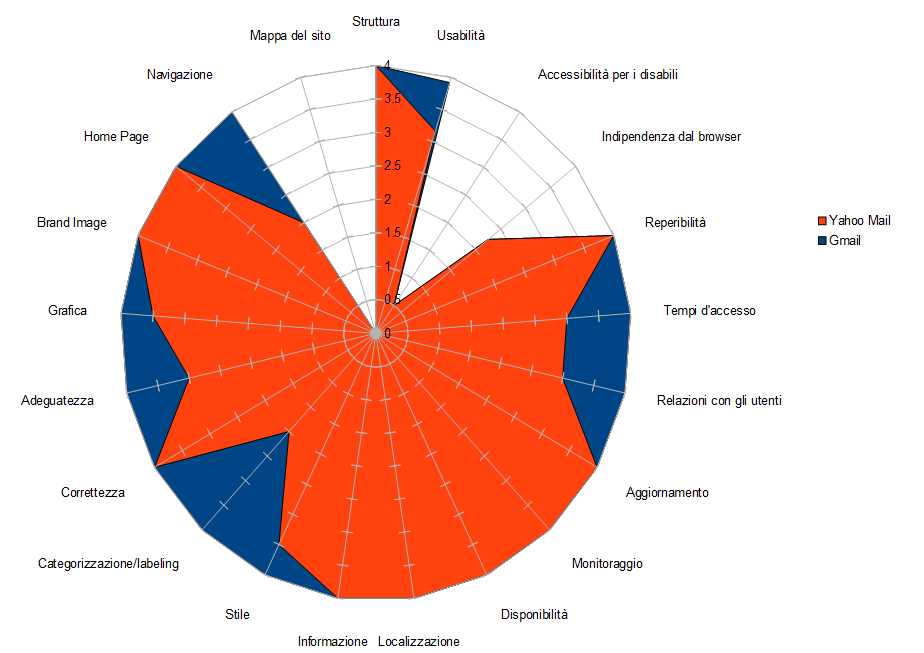
\includegraphics[scale=0.6]{radar_chart_sottocaratteristiche_filled.png}
			\end{center}
			\caption[Diagramma a stella (sottocaratteristiche)]{Diagramma a stella che confronta Gmail e Yahoo Mail secondo le sottocaratteristiche delle 7 caratteristiche individuate da  Polillo, con i voti delle Tabelle \ref{tab:valutazione_gmail} e \ref{tab:valutazione_yahoo}.}
			\label{fig:radar_chart_sottocaratteristiche}
		\end{figure}
